\documentclass[9pt]{beamer}
\usetheme{TUDOplain}
% workaround: provide commands not defiend by all bibtex styles
\providecommand{\btxandlong}{und}
\providecommand{\newblock}{}

\usepackage{pgfpages}
\setbeameroption{hide notes}

% link for how to present on mac with skim:
% https://gist.github.com/andrejbauer/ac361549ac2186be0cdb

% sourcing images
\providecommand{\source}{\\ \footnotesize \tugreen{Source:} \footnotemark}
\providecommand{\sourcefix}[1]{\\ \footnotesize \tugreen{Source:} [#1]}

\renewcommand{\caption}[1]{\\ \footnotesize{\captiongrey{#1}}}

\usepackage[english]{babel}
\usepackage[style=authortitle]{biblatex}
\addbibresource{../bibliography.bib}

% reformat footnotes very plain
\makeatletter
\renewcommand\@makefnmark{%
[\@thefnmark]}
\renewcommand\@makefntext[1]{%
  \noindent\tiny [\@thefnmark] #1}
\makeatother
% command for citing
\providecommand{\fcite}[1]{\footcite{#1}}
%

% basic utils
\usepackage[utf8]{inputenc}
\usepackage{enumerate}
\usepackage{graphicx}
\graphicspath{{../images/}}

\AtBeginSection[]{
  \begin{frame}
  \note[item]{placeholder}
  \vfill
  \centering
  \begin{beamercolorbox}[sep=8pt,center,shadow=true,rounded=true]{title}
    \usebeamerfont{title}\insertsectionhead\par%
  \end{beamercolorbox}
  \vfill
  \end{frame}
}

\usepackage{ifthen}
\usepackage{calc}
\usepackage{amsmath,amsfonts,amssymb}
\setbeamertemplate{navigation symbols}{}
%\setbeamertemplate{footline}{}
%\setbeamertemplate{footline}[frame number]{}
\setbeamertemplate{footline}{\small \vspace{-1ex} \vbox{ \insertframenumber /\inserttotalframenumber}}
%\setbeamertemplate{footline}{\fontsize{7pt}{7pt}\selectfont \vspace{-1ex} \vbox{ \insertframenumber /\inserttotalframenumber}}

\author{Matthias Jakobs}
\title{End-to-end Human Activity Recognition framework on Complex Video Datasets \\ Midterm presentation}
\date{\today}
\institute[TU Dortmund]{Pattern Recognition In Embedded Systems,\\ Department of Computer Science \\ LS XII, Technische Universität Dortmund}
%
% frame command
\newenvironment{myframe}[1][]{%
\begin{frame}%
\frametitle{#1}
% start footnote numbers with 1
\setcounter{footnote}{0}


}{%
\end{frame}%
}

\begin{document}
\begin{frame}

\titlepage

\end{frame}

\section{Motivation}
\begin{myframe}[Motivation]
    \begin{columns}[T]
        \begin{column}{.45\textwidth}
            \begin{itemize}
                \item Often: Human Activity Recognition approached separately from pose estimation
                \item Pose is used for HAR, but not learned jointly.
                \begin{itemize}
                    \item Shown to be very important feature
                \end{itemize}
                \item Idea: Both can benefit from each other
                \item Luvizon et al. \footnotemark~ propose approach for jointly learning both
            \end{itemize}
        \end{column}
        \footnotetext[1]{\cite{luvizon_2d/3d_2018}}
        \footnotetext[2]{\cite{reining_towards_2018}}
        \begin{column}{.45\textwidth}
            \begin{figure}
                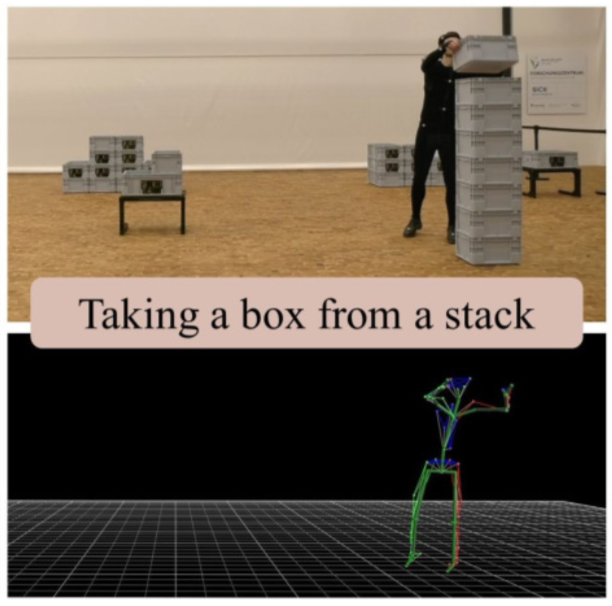
\includegraphics[width=.99\textwidth]{skeleton_har_example.png}
                \sourcefix{2}
            \end{figure}
        \end{column}
    \end{columns}
\end{myframe}

\tableofcontents

\section{Method}

\begin{myframe}[Method - Overview]
	\begin{columns}[T]
        \begin{column}{.45\textwidth}
            \begin{itemize}
                \item \textbf{Multitask Deep HAR}\footnotemark
                \begin{itemize}
                    \item Jointly train pose and action recognition
                    \item Pre-train pose estimation part, then fine-tune end-to-end
                    \item \textit{Soft-argmax}\footnotemark~makes end-to-end learning possible
                \end{itemize}
            \end{itemize}
        \end{column}
        \footnotetext[1]{\cite{luvizon_2d/3d_2018}}
        \footnotetext[2]{\cite{luvizon_human_2017}}
        \begin{column}{.45\textwidth}
            \begin{figure}
                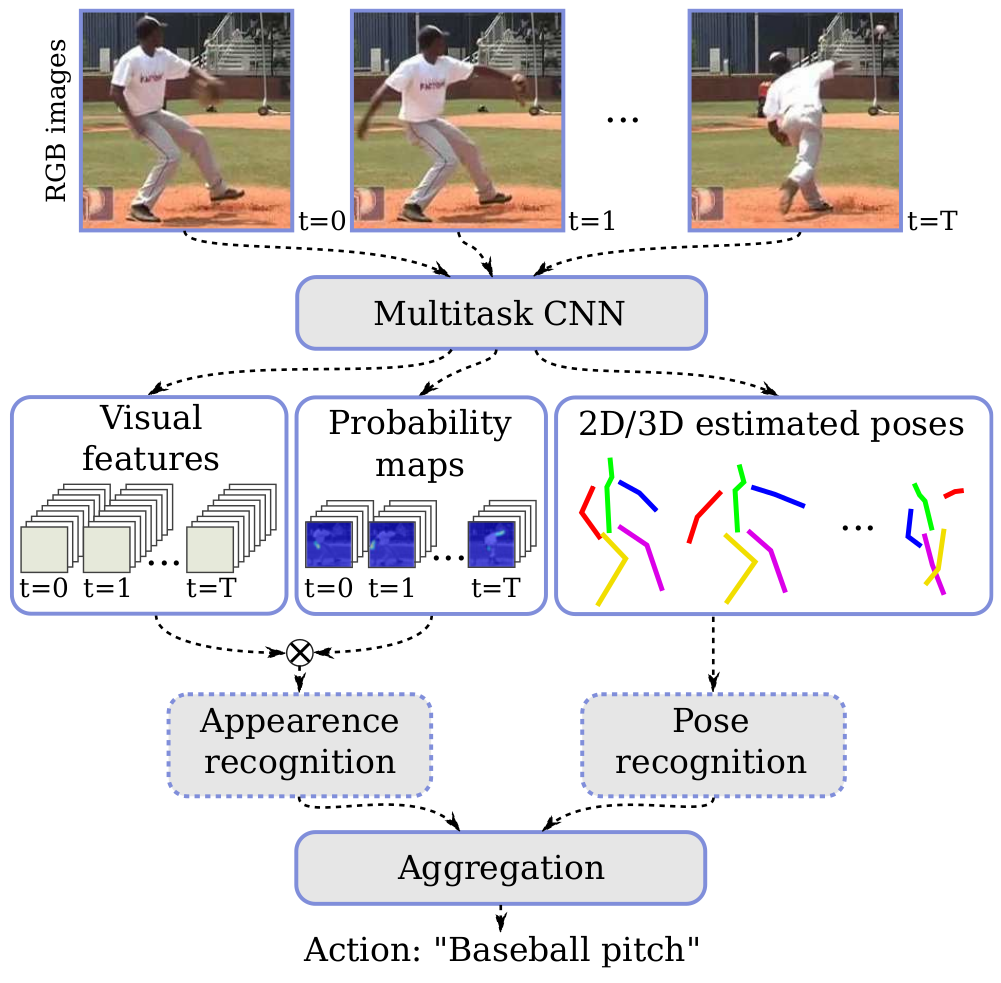
\includegraphics[width=.99\textwidth]{endtoend-concept.png}
                \sourcefix{1}
                %\caption{Complete network pipeline.}
            \end{figure}
        \end{column}
        \end{columns}
    \end{myframe}

\begin{myframe}[Method - Softargmax]
	\begin{columns}[T]
        \begin{column}{.45\textwidth}
            \begin{itemize}
                \item According to authors: Postprocessing necessary
                \item Propose \textbf{Soft-argmax} \footnotemark ~ in previous work
                \item Computes expectations on probability maps
                \item Fully differentiable
            \end{itemize}
        \end{column}
        \footnotetext[1]{\cite{luvizon_human_2017}}
        \footnotetext[2]{\cite{luvizon_2d/3d_2018}}
        \begin{column}{.45\textwidth}
            \begin{figure}
                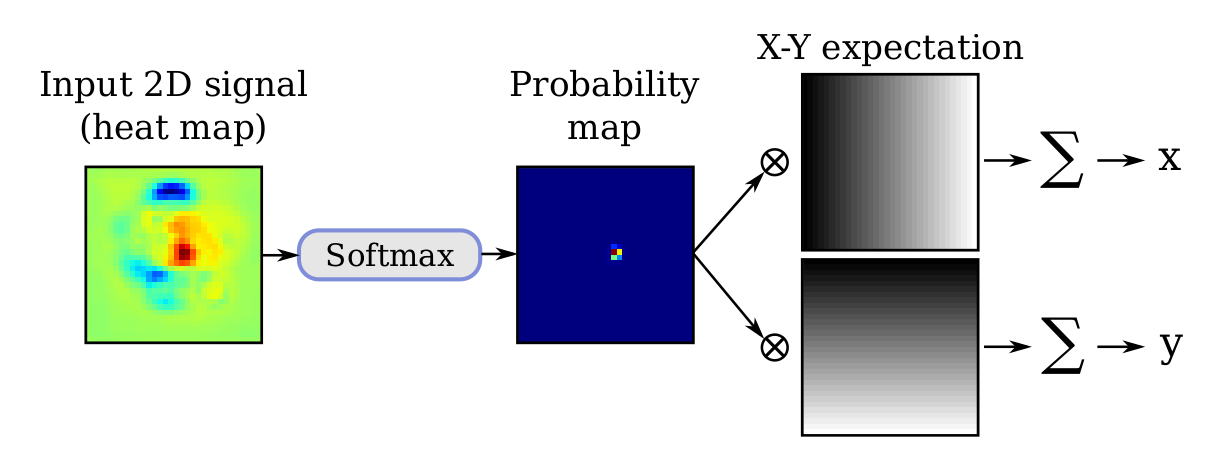
\includegraphics[width=.99\textwidth]{softargmax.png}
                \sourcefix{1}
                %\caption{Complete network pipeline.}
            \end{figure}
        \end{column}
	\end{columns}
\end{myframe}

\begin{myframe}[Method - Architecture]
    \begin{columns}[T]
        \begin{column}{.45\textwidth}
            \begin{itemize}
                \item \textit{Feature Extractor - Stem}
                \begin{itemize}
                    \item Based on Inception v4 \footnotemark
                    \item Uses \textbf{Depthwise separate convolutional layer}\footnotemark\footnotemark
                    \begin{itemize}
                        \item Used when high number of filters needed
                        \item Needs fewer parameters
                        \item Needs fewer matrix multiplications
                    \end{itemize}
                \end{itemize}
            \end{itemize}
        \end{column}
        \begin{column}{.45\textwidth}
            \begin{figure}
                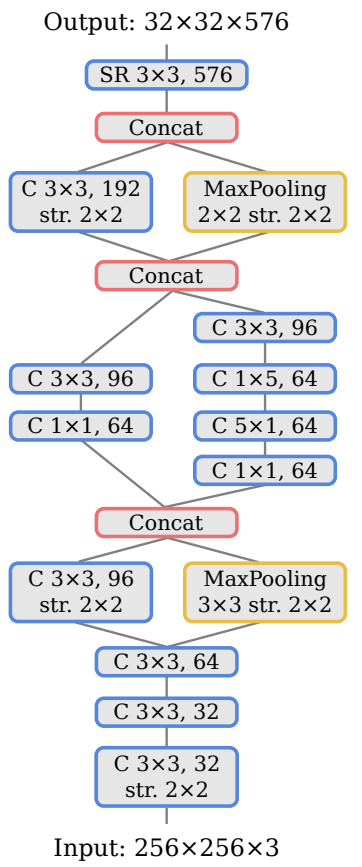
\includegraphics[width=.45\textwidth]{luvizon_stem.png}
                \sourcefix{4}
            \end{figure}
        \end{column}
	\end{columns}
    \footnotetext[1]{\cite{szegedy_inception-v4_2017}}
    \footnotetext[2]{\cite{sifre_rigid-motion_2014}}
    \footnotetext[3]{\cite{chollet_xception:_2017}}
    \footnotetext[4]{\cite{luvizon_2d/3d_2018}}
\end{myframe}

\begin{myframe}[Method - Depthwise separable convolution]
    \begin{itemize}
        \item Depthwise: $n$ filters of size $a \times a \times 1$
        \item Pointwise: $m$ filters of size $1 \times 1 \times n$
        \item Comparison:
        \begin{itemize}
            \item Regular convolution: $n \cdot m \cdot a^2$ parameters
            \item DSC: $n \cdot (m + a^2)$ parameters
        \end{itemize} 
    \end{itemize}

    \begin{figure}
        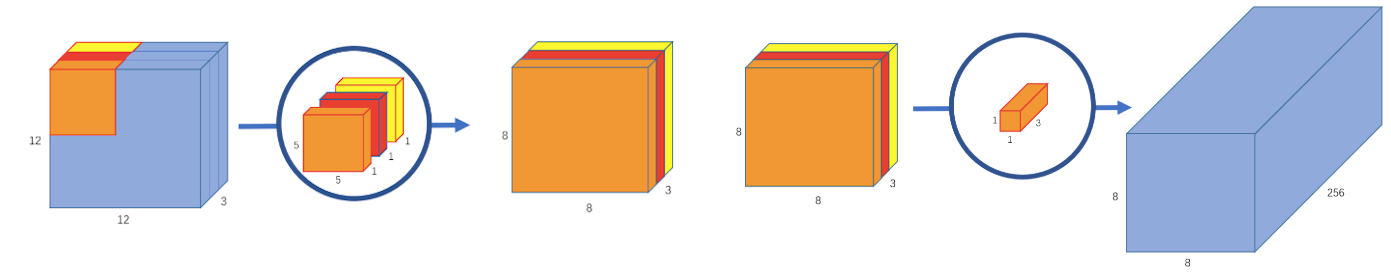
\includegraphics[width=.99\textwidth]{depthwise-visualization.png}
        \sourcefix{1}
    \end{figure}

    \footnotetext[1]{\url{https://towardsdatascience.com/a-basic-introduction-to-separable-convolutions-b99ec3102728}}
\end{myframe}


\begin{myframe}[Method - Pose Model]
	\begin{columns}[T]
        \begin{column}{.45\textwidth}
            \begin{itemize}
                \item Two paths in the network for action recognition
                \item \textit{Pose Model}
                \begin{itemize}
                    \item Arrange joint values over time in 2D matrix
                    \item Action heatmaps
                    \begin{itemize}
                        \item Through softmax: action probabilities
                    \end{itemize}
                \end{itemize}
            \end{itemize}
        \end{column}
        \begin{column}{.45\textwidth}
            \begin{figure}
                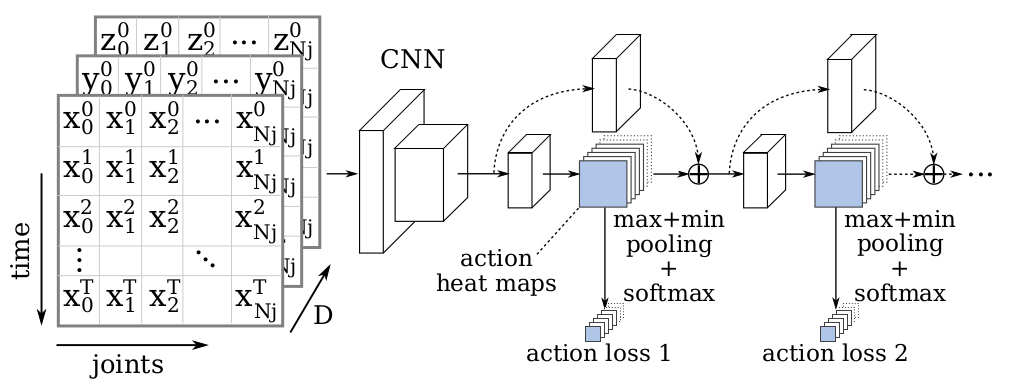
\includegraphics[width=.99\textwidth]{jointsovertime.png}
                \sourcefix{1}
            \end{figure}
        \end{column}
	\end{columns}
    \footnotetext[1]{\cite{luvizon_2d/3d_2018}}
\end{myframe}

\begin{myframe}[Method - Visual Model recognition]
    	\begin{columns}[T]
        \begin{column}{.45\textwidth}
            \begin{itemize}
                \item \textit{Visual Model recognition}
                \begin{itemize}
                    \item Combination of visual features and joint positions
                    \item Then: Identical architecture to pose recognition part
                \end{itemize}
                \item \textit{Aggregation}
                \begin{itemize}
                    \item Combine Pose Model and Visual Model results for final result
                    \item \textit{Categorical cross-entropy}
                \end{itemize}
            \end{itemize}
        \end{column}
        \begin{column}{.45\textwidth}
            \begin{figure}
                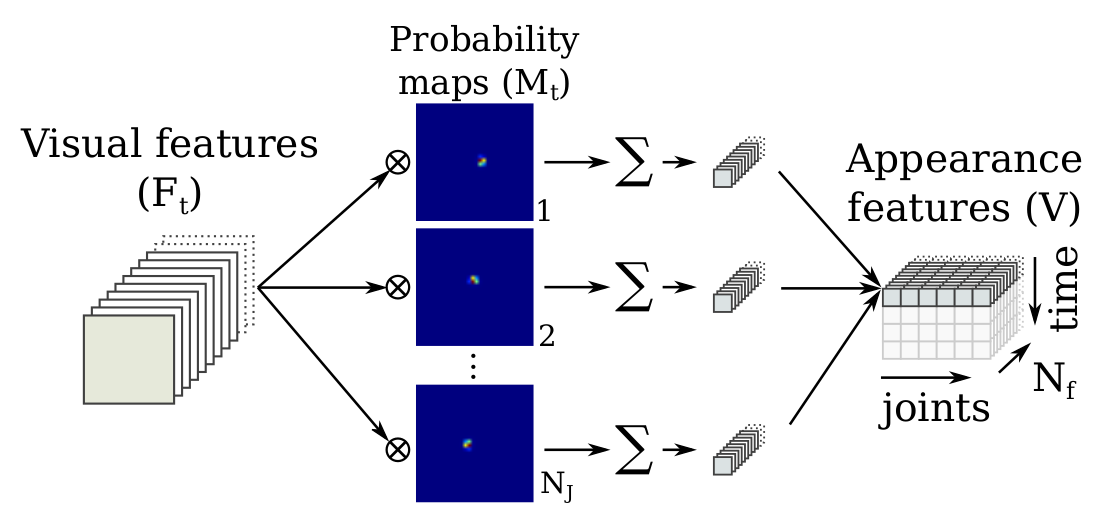
\includegraphics[width=.99\textwidth]{appearance-features.png}
                \sourcefix{1}
            \end{figure}
        \end{column}
	\end{columns}
    \footnotetext[1]{\cite{luvizon_2d/3d_2018}}
\end{myframe}

\begin{myframe}[Method - Extensions]
    \begin{itemize}
        \item Reimplementation in PyTorch \fcite{paszke_automatic_2017}
        \begin{itemize}
            \item Evaluate against JHMDB \fcite{jhuang_towards_2013}
        \end{itemize}
        \item Experimentation
        \begin{itemize}
            %\item Better incorporation of temporal dimension \fcite{pavllo_3d_2019}
            \item Ablation study to determine the choice of certain parameters
            \item Combined loss function of pose and action for \emph{real} end-to-end training
            \item Different representation of temporal information (next slide)
        \end{itemize}
    \end{itemize}
\end{myframe}

\begin{myframe}[Method - Different temporal representation]
    \begin{figure}
        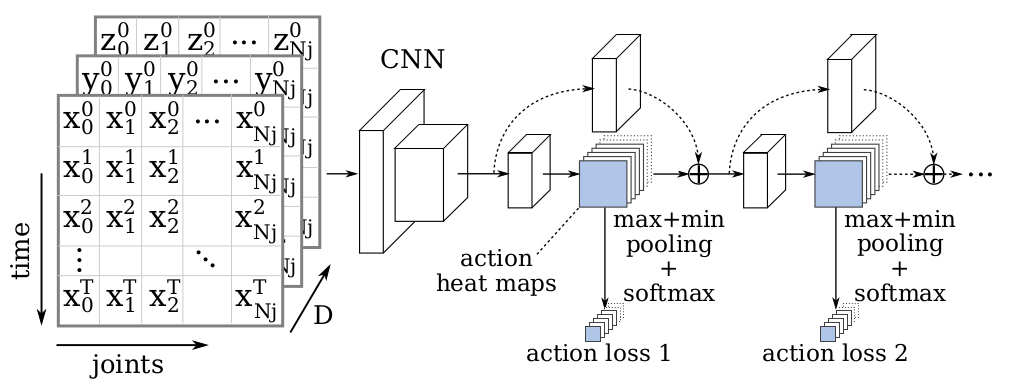
\includegraphics[width=.65\textwidth]{jointsovertime.png}
        \caption{Approach used by \footnotemark. Convolution over all sensors at once. \sourcefix{1}}
    \end{figure}
    \begin{figure}
        \includegraphics[width=.65\textwidth]{sensor-time.png}
        \caption{Impression of pixel coordinates of joints over time \source}
    \end{figure}
    \footnotetext[1]{\cite{luvizon_2d/3d_2018}}
    \footnotetext[2]{\url{https://avtech.com/articles/wp-content/uploads/2015/06/Intro.-Pic.png}}
\end{myframe}

\section{Datasets}
\begin{myframe}[2D Pose Datasets]
  \note[item]{placeholder}
  \begin{columns}[T]
      \begin{column}{.48\textwidth}
          \begin{itemize}
              \item \textbf{MPII Human Pose\footnotemark}
              \begin{itemize}
                  \item 40,000 annotated images
                  \item Single and multi person
                  \item Over 401 different activities
              \end{itemize}
          \end{itemize}
      \end{column}
      \footnotetext[1]{\cite{andriluka_2d_2014}}
      \begin{column}{.48\textwidth}
          \begin{figure}
              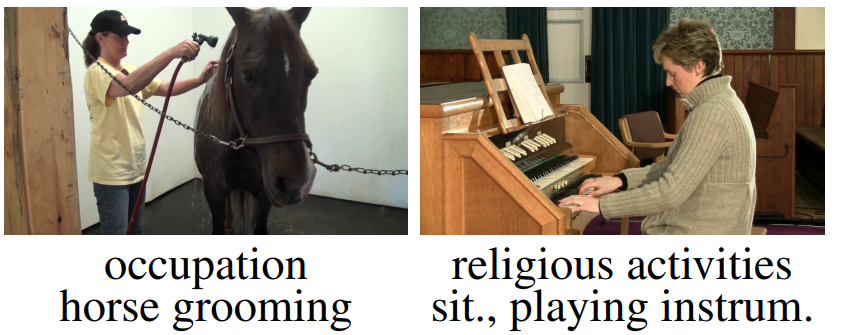
\includegraphics[width=0.99\textwidth]{mpii.png}
              \sourcefix{1}
          \end{figure}
      \end{column}
  \end{columns}
\end{myframe}

\begin{myframe}[Action Recognition Datasets]
  \begin{columns}[T]
      \begin{column}{.48\textwidth}
          \vspace{20px}
          \begin{itemize}
              \item \textbf{Penn Action\footnotemark}
              \begin{itemize}
                  \item 2,400 video clips of 15 actions
                  \item Limited number of actions (mainly sport)
              \end{itemize}
          \end{itemize}
      \end{column}
      \footnotetext[1]{\cite{zhang_actemes_2013}}
      \begin{column}{.48\textwidth}
          \begin{figure}
              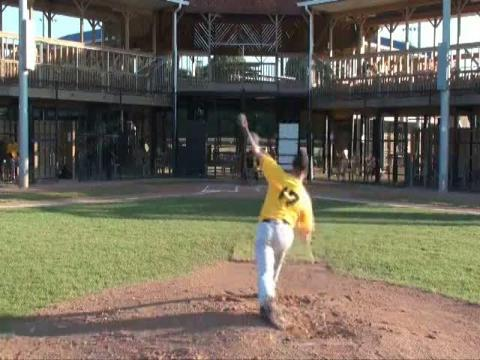
\includegraphics[height=45px]{pa-01.jpg}
              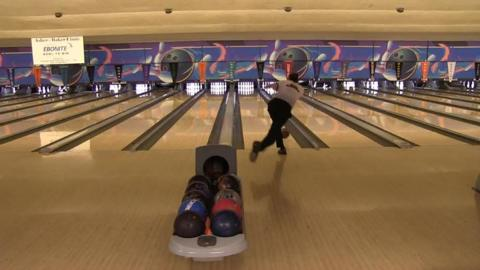
\includegraphics[height=45px]{pa-02.jpg}
              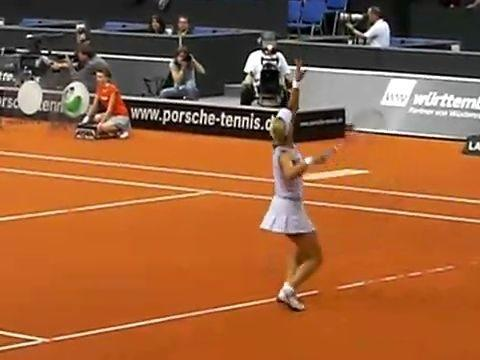
\includegraphics[height=45px]{pa-03.jpg}
              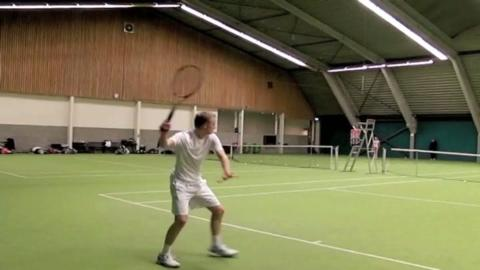
\includegraphics[height=45px]{pa-04.jpg}
              \source
          \end{figure}
      \end{column}
  \end{columns}
  \footnotetext[2]{\url{https://upenn.app.box.com/v/PennAction}}
\end{myframe}

\begin{myframe}[Action Recognition Datasets]
  \begin{columns}[T]
      \begin{column}{.48\textwidth}
          \begin{itemize}
              \item \textbf{JHMDB\footnotemark}
              \begin{itemize}
                  \item Fully-annotated subset of HMDB
                  \begin{itemize}
                      \item 2D pose
                      \item Subject segmentation maps
                      \item Optical flow
                  \end{itemize}
                  \item 928 clips of 21 actions
                  \item Can be used for end-to-end training
              \end{itemize}
          \end{itemize}
      \end{column}
      \footnotetext[1]{\cite{jhuang_towards_2013}}
      \begin{column}{.48\textwidth}
          \begin{figure}
              \includegraphics[height=.55\textheight]{jhmdb.png}
              \centering
              \source
          \end{figure}
      \end{column}
  \end{columns}
  \footnotetext[2]{\url{http://jhmdb.is.tue.mpg.de/puppet_tool}}
\end{myframe}

\section{Experiments}
\begin{myframe}[Recreate experiments - Meassurements]
    % TODO: Cite all this
    \begin{itemize}
        \item 2D Pose estimation
        \begin{itemize}
            \item \textit{Probability of Correct Keypoints} with regards to head size (\textit{PCKh})
            \begin{itemize}
                \item Meassure distance between ground truth keypoint and estimation
                \item If smaller than ($\alpha \cdot \text{head bbox size}$): correctly estimated
                \item Used for highly articulated poses
                \item In literature: $\alpha \in \{0.2, 0.5\}$
            \end{itemize}    
            \item \textit{PCK} with regards to subject bounding box
            \begin{itemize}
                \item Problem with highly articulated poses
                \item Used whenever no head size given
                \item Can be computed from all datasets used
                \item $\alpha = 0.2$ used in literature
            \end{itemize}
        \end{itemize}
        \item Action recognition
        \begin{itemize}
            \item Simple accuracy meassurement in literature
            \item $F_1$ meassure not needed since all datasets are balanced w.r.t. classes
        \end{itemize}
    \end{itemize}
\end{myframe}

\begin{myframe}[Recreate experiments - 2D Pose estimation]
    \begin{itemize}
        \item Recreate results for using different parameters
        \item In general:
        \begin{itemize}
            \item More prediction blocks lead to higher accuracy
            \item Context maps yield slighly higher accuracy for small network
        \end{itemize}
    \end{itemize}
    \begin{figure}
        \begin{table}[]
            \small
            \begin{tabular}{|l|c|c|c|c|}
            \hline
             & \textbf{nr\_blocks} & \textbf{nr\_context} & \textbf{PCKh @ 0.5 (validation)} & \textbf{PCKh @ 0.5 (test)} \\ \hline
            \textbf{Own} & 2 & 0 & 80.96 &  \\
            \textbf{} & 2 & 2 & 81.56 &  \\
            \textbf{} & 4 & 0 & 83.22 &  \\
            \textbf{} & 4 & 2 & 82.97 &  \\
            \textbf{} & 8 & 0 & 84.67 &  \\
            \textbf{} & 8 & 2 & 84.66 & tbd \\ \hline
            \textbf{\footnotemark} & 8 & 2 & 89.00 & 91.2 \\ \hline
            \end{tabular}
        \end{table}
    \end{figure}
    \footnotetext[1]{\cite{luvizon_2d/3d_2018}}
\end{myframe}

\begin{myframe}[Recreate experiments - 2D pose estimation]
    \begin{figure}
        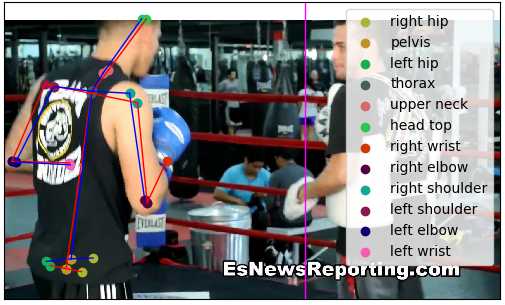
\includegraphics[height=.80\textheight]{mpii_8_positive.png}
        \centering
        \caption{\tugreen{Figure:} Positive example. Ground truth pose shown in red, estimated pose shown in blue.}
    \end{figure}
\end{myframe}

\begin{myframe}[Recreate experiments - 2D pose estimation]
    \begin{figure}
        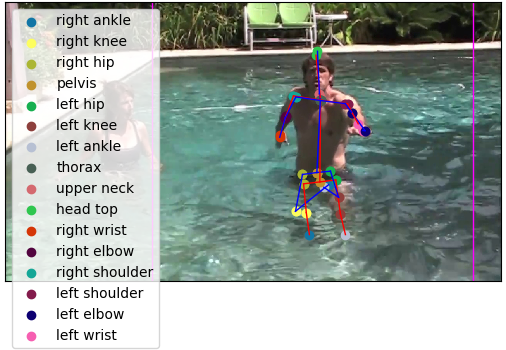
\includegraphics[height=.80\textheight]{mpii_8_negative.png}
        \centering
        \caption{\tugreen{Figure:} Negative example. Notice that the lower limbs are wrongly estimated due to the water.}
    \end{figure}    
\end{myframe}

\begin{myframe}[Recreate experiments]
    \begin{itemize}
        \item Penn Action HAR
        \item tbd
    \end{itemize}
\end{myframe}

\begin{myframe}[2D pose estimation on JHMDB]
    \begin{itemize}
        \item Used ground truth bounding boxes as in \footnotemark
        \item Additionally: \textit{PCK} w.r.t. upper body size (\textit{PCKu})
        \item Dataset more challenging because of video artifacts
    \end{itemize}
    \begin{figure}
        \begin{table}[]
            \small
            \begin{tabular}{|l|c|c|c|c|}
            \hline
             & \textbf{nr\_blocks} & \textbf{nr\_context} & \textbf{PCK @ 0.2 (test)} & \textbf{PCKu @ 0.2 (test)} \\ \hline
            \textbf{Own} & 2 & 0 & TODO &  \\
            \textbf{} & 2 & 2 & TODO &  \\
            \textbf{} & 4 & 0 & TODO &  \\
            \textbf{} & 4 & 2 & TODO &  \\
            \textbf{} & 8 & 0 & TODO &  \\
            \textbf{} & 8 & 2 & TODO &  \\ \hline
            \textbf{\footnotemark} &  &  & 81.60 &  \\ \hline
            \end{tabular}
        \end{table}
    \end{figure}
    \footnotetext[1]{\cite{luvizon_2d/3d_2018}}
    \footnotetext[2]{\cite{song_thin-slicing_2017}}
\end{myframe}

\begin{myframe}[HAR on JHMDB dataset]
    \begin{itemize}
        \item best jhmdb found: 87.9 percent \footnotemark
    \end{itemize}
    \footnotetext[1]{\cite{choutas_potion:_2018}}
\end{myframe}

\section{Conclusion}
\begin{myframe}[Conclusion]
    \begin{itemize}
         \item What is left to do
        \item TODO
    \end{itemize}
\end{myframe}

\begin{myframe}[Thank you]
    \note[item]{placeholder}
    \centering \Large
    \emph{Thank you for your time!}
\end{myframe}

\end{document}

